\section{Boomerang Design} \label{sec:design}

As previously discussed, the Boomerang protocol enhancement for Bitcoin is motivated by the need to hide the source from which transactions are introduced into the network. Furthermore, this should be done in a transparent way so that any other form of anonymous coin extension on top of Bitcoin (e.g., Zerocoin) can leverage the service for transaction anonymity. Boomerang is \emph{not} intended to support regular Bitcoin traffic; once a transaction becomes public knowledge, Boomerang no longer plays a role in its distribution. 

In the following sections we detail the core protocol and several important design and security tradeoffs that can be made in practice when using Boomerang. A formal analysis of the security and performance of Boomerang-enhanced Bitcoin is provided in Sections X and Y. 

\subsection{Boomerang Peer-to-Peer Network Design}
Boomerang peer discovery is done in a similar manner to the Bitcoin peer discovery process described above with a few exceptions. Boomerang nodes can also query Bitcoin nodes after connecting to the Bitcoin network. Boomerang nodes can also learn the address of other nodes by routing Boomerang messages. The Boomerang peer discovery methods are:

\begin{enumerate}
	\item User inputted addresses from command line or text file: If the user manually inputs address information, the client will attempt to connect to those Boomerang peers first.
	\item Node reads stored Boomerang addresses from previous sessions: Boomerang clients will attempt to connect to peers stored in the internal address database from the previous session.
	\item Nodes make a DNS request for Boomerang seed nodes: If there are no active nodes in the internal address database, then the client will perform a DNS lookup using hard-coded DNS servers for current seed nodes.
	\item Nodes connect to hard-coded seed addresses: If DNS lookups fail, then the client attempts to connect to hard-coded seed addresses.
	\item Nodes query Bitcoin network for Boomerang nodes: The client sends Boomerang connection requests to nodes on the Bitcoin network.
	\item Nodes utilize callback addresses: After receiving a Boomerang connection request from a remote node, the client node can use the callback address to connect to the remote node and exchange address database information.
	\item Nodes receive relayed addresses: After receiving new address information and verifying validity of the address, a node will randomly pick a few nodes in the internal database and relay the new address information.
	\item Nodes will self broadcast periodically: Similarly to relayed addresses, periodically Boomerang clients will randomly pick a few nodes in the internal database and relay its own address information.
	\item Boomerang messages: The destination of a Boomerang message must be a Boomerang node. The client can then request a connection with the destination node and exchange address database information.
\end{enumerate}

\subsection{Broadcast Protocol}

At the heart of the Bitcoin protocol is the ability to encode new transactions as Boomerang messages and then ripple them throughout the network. We describe the complete procedure for message encoding, {\sf EncodeTransaction}, in Algorithm \ref{alg:encode}, where the notation contained therein is defined in Table \ref{tab:notation}. An encoded Boomerang message has a very well-defined format, as shown in Figure \ref{fig:boomerang_message}. In particular, the message is composed of the following:
\begin{enumerate}
	\item A potentially re-encrypted seed. By the description of {\sf EncodeTransaction}, it is required that the public-key encryption scheme used to mask these seeds has the same domain and range. This is needed because the decrypted seed for one hop will be used as decrypted seed on the previous hop, very much like onion layers of encryption.
	\item An encrypted address vector that is used by each hop to learn the next hop in the circuit without learning any other information about the nodes in the circuit. More specifically, a router can only learn about the immediate source and destination of a Boomerang message (the security and anonymity implications of this are discussed in the following section).
	\item A potentially re-encrypted transaction message block. This block either stores the encrypted transcaction, where the encryption is done by XORing with a pseudorandom bit string generated by the decrypted seed value, or the plaintext transaction that is to be broadcast throughout the network.
\end{enumerate}

\begin{table*}[ht!]
\begin{center}
\caption{Boomerang Protocol Notation}
	\begin{tabular}{|l|l|}\hline
	\textbf{Symbol} & \textbf{Description} \\ \hline
	~ & ~ \\
	~ & ~ \\
	~ & ~ \\ \hline
	\end{tabular}
\end{center}
\end{table*}

\begin{figure}[ht!]
\begin{center}
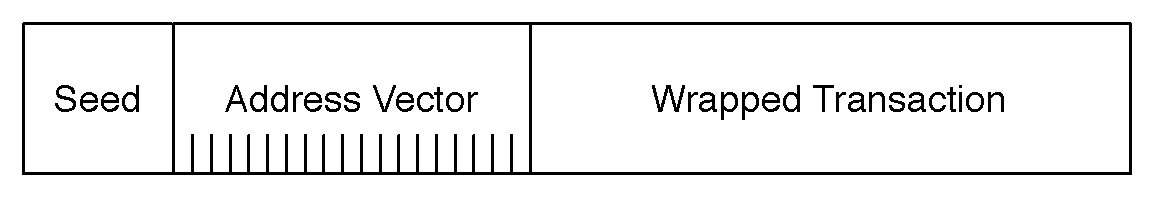
\includegraphics[scale=0.4]{./images/boomerang_message.pdf}
\caption{Boomerang message encoding.}
\label{fig:boomerang_message}
\end{center}
\end{figure}

The procedure to handle Boomerang messages, {\sf BoomerangMessageHandler}, is provided in Algorithm \ref{alg:handler}. 

\begin{algorithm*}[t!]
\caption{{\sf EncodeTransaction}($T$)}
\label{alg:encode}
\begin{algorithmic}[1]

\For{$i = 1$ to $W$}
	\State $\bar{T} := T$
	\State $s \gets \{0,1\}^{\tau}$
	\For{$j = 1$ \textbf{to} $D_i$}
		\State $p := \mathsf{PRG}(s)$
		\State $\bar{T} := \bar{T} \oplus p$
		\State $s \gets E_{pk_{i,j}}(s)$
	\EndFor

	% populate the address vector
	\State $\mathsf{index} \gets \{0,\dots,2D_i\}$ % random address vector index
	\State $\mathsf{AV} := [2D_i]$ % address vector
	\For{$j = D_i$ \textbf{downto} $2$}
		\State $\mathsf{AV}[\mathsf{index}] := E_{pk_{i,j}}(\mathsf{addr}_{D_j})$
		\State $\mathsf{index} := \mathsf{index} + 1 (\mod N_m)$
		\State $\mathsf{AV}[\mathsf{index}] := E_{pk_{i,j}}(\mathsf{addr}_{D_{j-1}})$
		\State $\mathsf{index} := \gets \{0,\dots,2D_i\}$
		\While {$\mathsf{index} \mod 2 \not= 0$ \text{ and } $\mathsf{AV}[\mathsf{index}] \not= \bot \text{ and } \mathsf{AV}[\mathsf{index + 1 (\mod D_i)}] \not= \bot$}
			\State $\mathsf{index} \gets \{0,\dots,2D_i\}$
		\EndWhile
	\EndFor

	\State $M := \mathsf{Pack}(s, \mathsf{AV}, \bar{T})$
	\State $\mathsf{Transmit}(M)$
\EndFor

\end{algorithmic}
\end{algorithm*}

\begin{algorithm*}[t!]
\caption{{\sf BoomerangMessageHandler}($j$, $M$)}
\label{alg:handler}
\begin{algorithmic}[1]

\State $s := D_{sk_{j}}(M[0])$
\State $\bar{T} := M[2] \oplus PRG(s)$
\If {$\bar{T}$ is a well formed transaction}
	\State $\mathsf{Broadcast}(\bar{T})$ to the Bitcoin network
\ElsIf {$\bar{T}$ destination address is $\mathsf{addr}_j$}
	\State Discard $\bar{T}$; return;
\Else
	\State $\mathsf{AV} := M[1]$
	\State $i := 1$
	\While {$i < \mathsf{len}(\mathsf{AV})$}
		\State $\mathsf{addr}_{src} := D_{pk_j}(AV[j])$
		\If {$\mathsf{addr}_{src} = \mathsf{addr}_j$}
			\State $\mathsf{addr}_{dst} := D_{pk_j}(AV[j + 1])$
			\State $M := \mathsf{Pack}(s, \mathsf{AV}, \bar{T})$
			\If {$|Buffer| \geq B$}
				\State $\mathsf{Transmit}(M)$
			\Else
				\State $B.add(M)$
			\EndIf
		\Else
			\State $i := i + 2$
		\EndIf
	\EndWhile
\EndIf

\end{algorithmic}
\end{algorithm*}

% TODO: cover traffic generation, mix delay

Similar to the Tarzan P2P mixnet, a critical part of the Boomerang protocol is the inclusion of cover traffic that is indistinguishable from legitimate encoded Boomerang transaction messages \cite{tarzan}. This traffic is needed for two reasons: (1) to keep legitimate transactions moving through mixnet circuits, and (2) to obfuscate the flow of legitimate transactions through the network. To support this cover traffic with minimal changes to the protocol, nodes in the network will \emph{reuse} and \emph{re-encode} old transactions to be sent throughout the network, with the exception that the destination node for the mixnet circuit (as specified in the {\sf EncodeTransaction} procedure) will be the same as the sender. This is because the sender can easily discover when a transaction message has looped through the network and back to themselves, at which point they can then simply discard the transaction. Clearly, the rate at which this cover traffic is generated plays a critical role in the overall performance of the system when using Boomerang. We discuss the selection of parameters that achieve optimal performance without sacrificing security in Section 5. 

\subsection{Cryptographic Primitives}

% TODO: PRG, PK-encryption, etc

Based on the {\sf EncodeTransaction} and {\sf BoomerangMessageHandler} procedures, we require the following cryptographic primitives to support Boomerang messages:
\begin{enumerate}
	\item Uniform domain and range public-key encryption without ciphertext expansion, and
	\item Deterministic PRG whose input is an element in the range specified by the public-key encryption scheme.
\end{enumerate}

To satisfy the first primitive, we chose the standard RSA cryptosystem. While ElGamal has the ideal property that plaintext and ciphertext elements are members of the same group $\mathbb{Z}_p$ for some sufficiently large prime $p$, the ciphertext actually consists of a pair of group elements, and thus does not satisfy the ciphertext expansion property. Also, while RSA-OAEP is the only known CCA-secure variant of RSA (in the Random Oracle model), the input plaintext is strictly less than the output ciphertext due to the applied padding. Therefore, this does not achieve the first property that function domain and range are equivalent. 

% TODO: rsa & prg

% \begin{figure}[ht!]
% \begin{center}
% 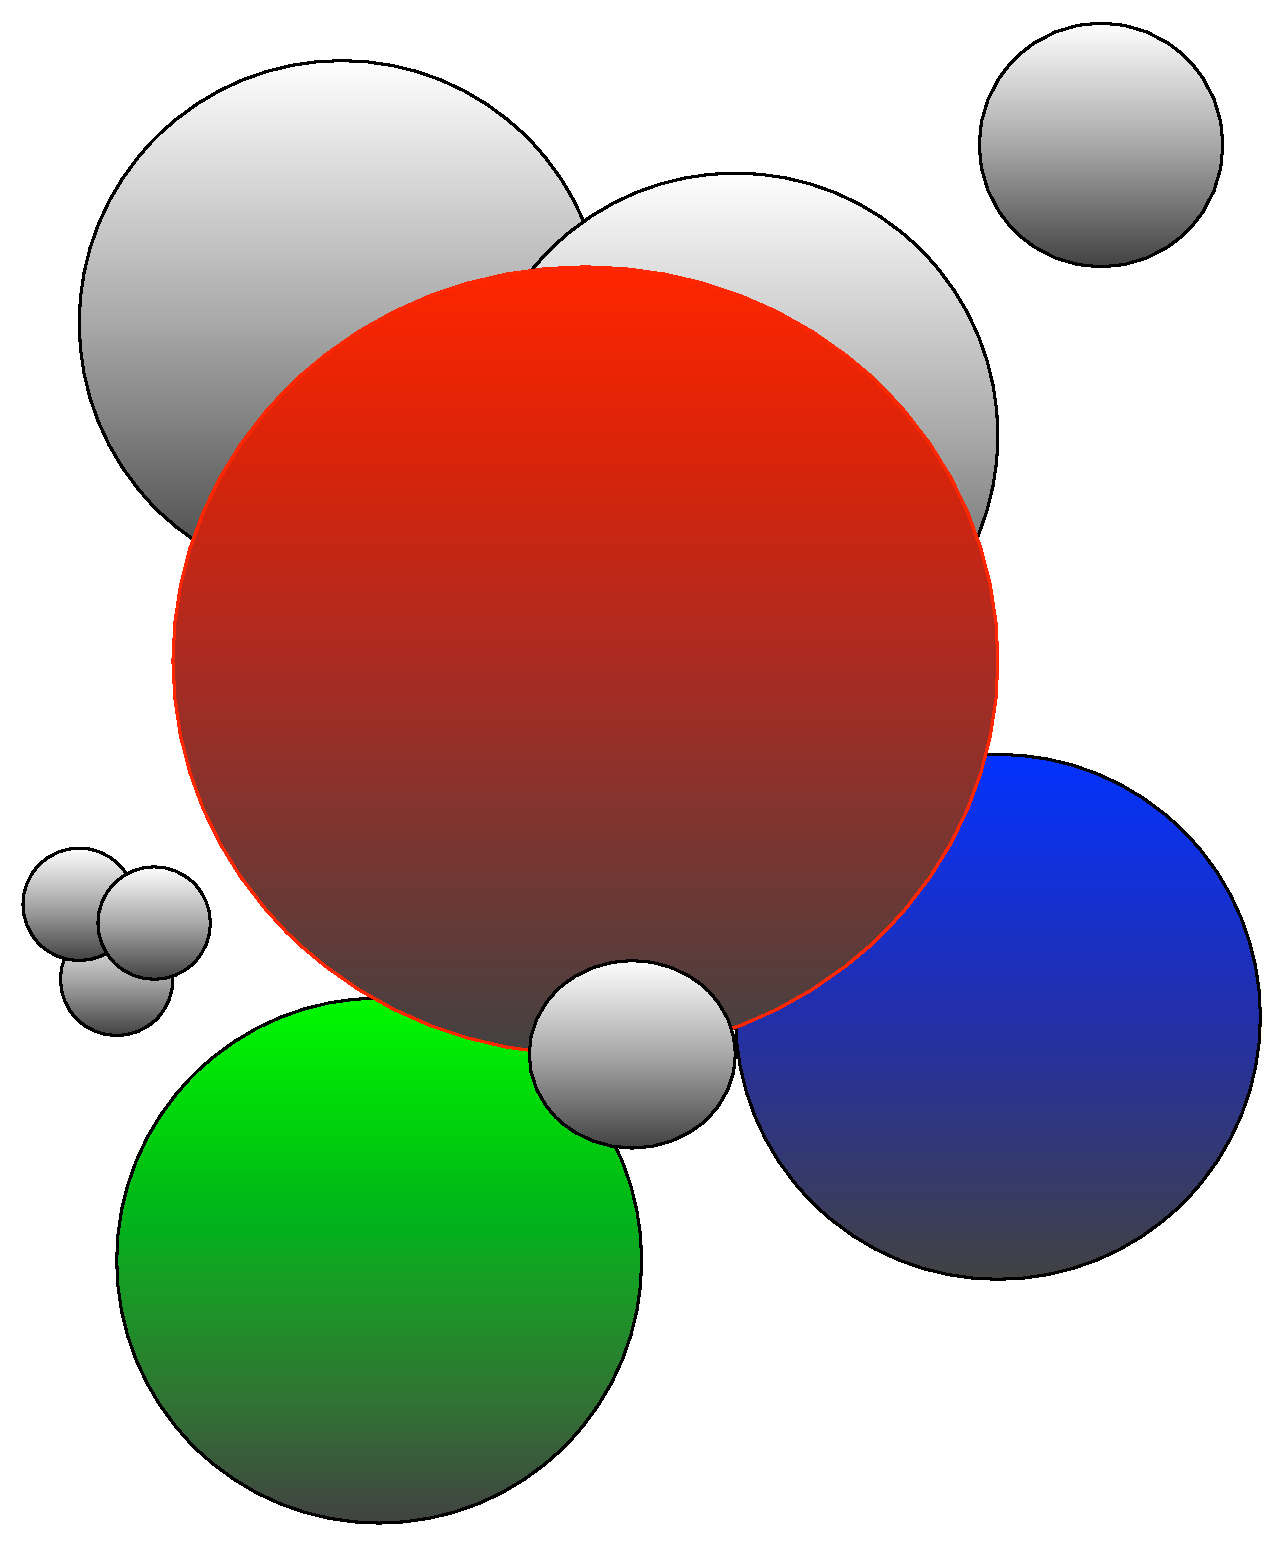
\includegraphics[scale=0.25]{./images/boomerang_clusters.pdf}
% \caption{TODO}
% \label{fig:boomerang_clusters}
% \end{center}
% \end{figure}

\subsection{Node Verification}
Boomerang clients need to validate addresses in the internal database. In order to validate addresses, Boomerang messages will be sent through un-validated addresses as well as validated addresses. If the local client correctly decrypts the Boomerang message, the nodes along the message’s route are marked as verified with a timestamp in the internal database. Boomerang clients will only relay address information from verified addresses.

% TODO: gossip protocol, duration of Boomerang public/private key pairs, what else?

% To protect against fake entries, Tarzan differentiates between un- validated and validated addresses in the peer-discovery and selec- tion process. Honest nodes only propagate validated addresses and only select mimics from their set of validated addresses.


% Furthermore, a global eavesdropper that watches nodes gossip
% can record the α nodes we assume each learns from the total set
% of size n. Therefore, only α possible nodes could have initiated
% a tunnel establishment request to a colluding malicious node.  In
% general, for any α < n, this discovery-profiling attack leaks some 10
% information and thus should be avoided.
